\newcommand{\teta}{\tilde{\eta}}

Incompressible flow represents the zero-Mach number limit of fluid
flow---no compressibility effects are modeled.  We can extend the
ideas of incompressibe flow to allow us to model some compressibility
effects, giving rise to low Mach number methods.

\section{Low Mach divergence constraints}

The key idea in solvers for low Mach number flows is that, as a fluid
element advects, its pressure remains the same as the background
state.  For an atmosphere, this background state is a hydrostatic
profile.  For a smallscale combustion flow, this background state is a
spatially constant pressure (and constaint-in-time if the domain is
open).

We can derive the constraint on the velocity field by considering the
Lagrangian derivative of the pressure---this captures the change in
pressure of a fluid element as it moves through the domain.



\section{Extending the incompressible algorithm}

\subsection{Variable-coefficient elliptic equation}

We now need to solve an elliptic equation of the form:
\begin{equation}
\nabla \cdot (\eta \nabla \phi) = f
\end{equation}

If we denote the discrete divergence and gradient operators as $D$ and $G$,
then our operator will be $L_\eta \equiv D \eta G$.  If we wish to
use a cell-centered discretization for $\phi$, then using a standard 
centered-difference for $D$ and $G$ will result in a stencil that reaches
two zones on either side of the current zone.  This can lead to an
odd-even decoupling. \MarginPar{cite the appropriate Bell paper}

\MarginPar{there is a Pao and Colella (or Pao's thesis?) that also 
discusses issues with cell-centered}

Instead, we again use an approximate projection.  We discretize the
variable-coefficient Laplacian as:
\begin{align}
(L_\eta \phi)_{i,j} = 
 & \frac{\eta_{i+1/2,j} (\phi_{i+1,j} - \phi_{i,j}) -
        \eta_{i-1/2,j} (\phi_{i,j} - \phi_{i-1,j})}{\Delta x^2} + \nonumber \\
 & \frac{\eta_{i,j+1/2} (\phi_{i,j+1} - \phi_{i,j}) -
        \eta_{i,j-1/2} (\phi_{i,j} - \phi_{i,j-1})}{\Delta y^2}
\label{lm:eq:lap}
\end{align}

We can define the interface values of $\eta$ as the averages of the
cell-centered values.  Our elliptic equation is then 
\begin{equation}
(L_\eta \phi)_{i,j} = f_{i,j}
\end{equation}

The relaxation method for this operator again relies on isolating
$\phi_{i,j}$, yielding:
\begin{equation}
\phi_{i,j} = \frac{\teta_{i+1/2,j}\phi_{i+1,j} + \teta_{i-1/2,j}\phi_{i-1,j} +
                   \teta_{i,j+1/2}\phi_{i,j+1} + \teta_{i,j-1/2}\phi_{i,j-1} -
                   f_{i,j} } 
                  {\teta_{i+1/2,j} + \teta_{i-1/2,j} + 
                   \teta_{i,j+1/2} + \teta_{i,j-1/2}}
\label{lm:eq:smooth}
\end{equation}
with the shorthand that $\teta_{i\pm1/2,j} = \teta_{i\pm1/2,j}/\Delta x^2$
and $\teta_{i,j\pm1/2} = \teta_{i,j\pm1/2}/\Delta y^2$.

To put this into our multigrid framework, there are three changes we
need to make:
\begin{itemize}
\item The smoothing function needs to implement the more general smoothing
described by Eq.~\ref{lm:eq:smooth}.

\item The residual function needs to compute $(L_\eta \phi)_{i,j}$ according
to Eq.~\ref{lm:eq:lap}, and then $r_{i,j} = f_{i,j} - (L_\eta \phi)_{i,j}$.

\item The coefficients, $\eta$ should be averaged to the edges on the fine
grid and then restricted down the multigrid hierarchy as edge-based 
quantities.
\end{itemize}

\subsection{Test problem}

\subsubsection{Periodic}

To test the solver, we need to devise a problem with a known analytic
solution.  The easiest way to do this is to pick an $\eta(x)$ and
$\phi$ and then do the divergence and gradients to find the required
righthand side, $f$.  We'll use periodic BCs, and for our
equation $\nabla \cdot ( \eta \nabla \phi ) = f$, the following
provide a well-posed test problem:
\begin{align}
\phi^\mathrm{true} &= \sin(2 \pi x) \sin(2\pi y) \nonumber \\
\eta &= 2 + \cos(2\pi x) \cos(2\pi y)  \label{eq:vc:lap}
\\
f &= -16.0 \pi^2 \left [ \cos(2\pi x)\cos(2\pi y) + 1 \right ] \sin(2\pi x)\sin(2 \pi y) \nonumber
\end{align}

There is an important caveat when dealing with a purely-periodic
problem.  Since there is no boundary values to ``anchor'' the solution,
it is free to float.  Solving the elliptic problem will give use the
correct $\nabla \phi$, but the average of $\phi$ over the domain is 
unconstrained.  For our algorithms, it is $\nabla \phi$ that matters
(that is the forcing term that enters into the momentum equation).

When for checking convergence, we want to compare to the exact solution.
We therefore normalize $\phi$ by subtracting off its average value before
computing the norm of the error with respect to the exact solution:
\begin{equation}
\epsilon = \| \phi_{i,j} - \bar{\phi} - \phi^\mathrm{true}_{i,j} \|
\end{equation}.
where
\begin{equation}
\bar{\phi} = \frac{1}{N_x N_y} \sum_{i,j} \phi_{i,j}
\end{equation}
As discussed in \S~\ref{sec:multigrid:other}, this can arise if
the discrete form the righthand side, $f_{i,j}$ does not sum exactly
to zero.  Figure~\ref{fig:mg_vc} shows the solution to this problem
with a $512^2$ grid. and the convergence of the solver described
here is shown in Figure~\ref{fig:mg_vc_converge}.

\begin{figure}[t]
\centering
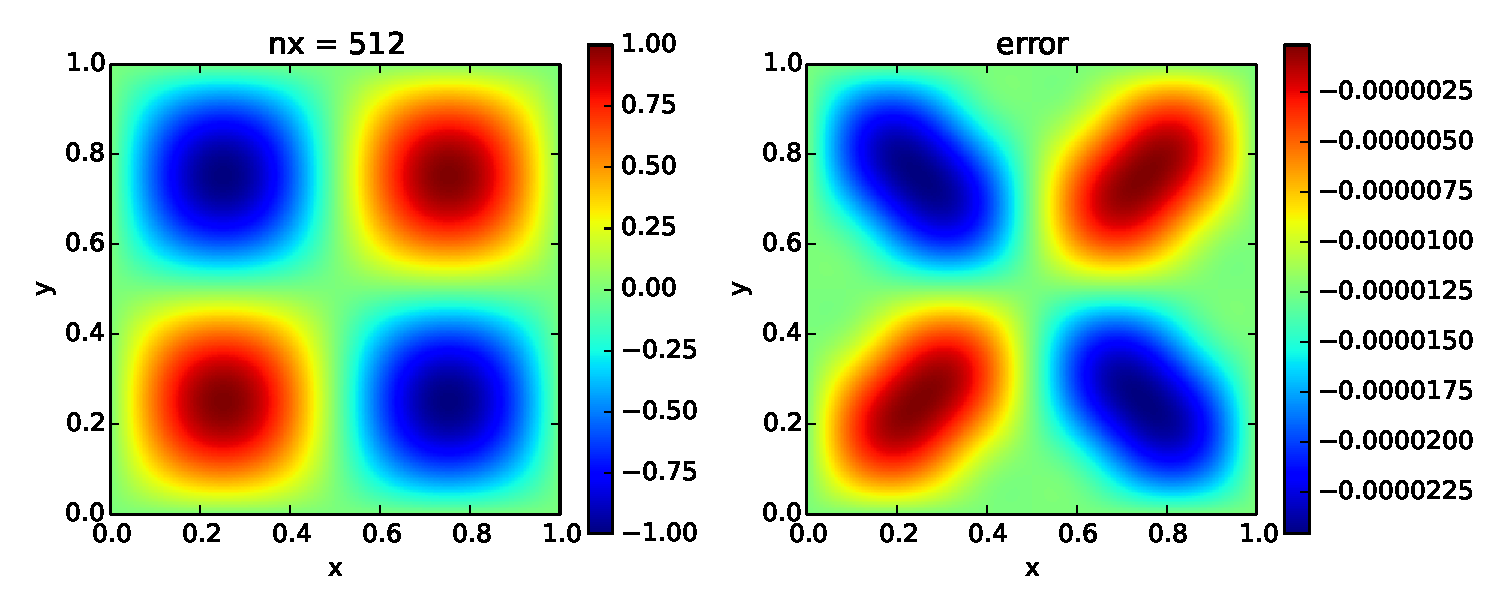
\includegraphics[width=\linewidth]{mg_vc_periodic_test}
\caption{\label{fig:mg_vc} Solution and error to the variable-coefficient 
Poisson problem defined in Eq.~\ref{eq:vc:lap}}.
\end{figure}

\begin{figure}[t]
\centering
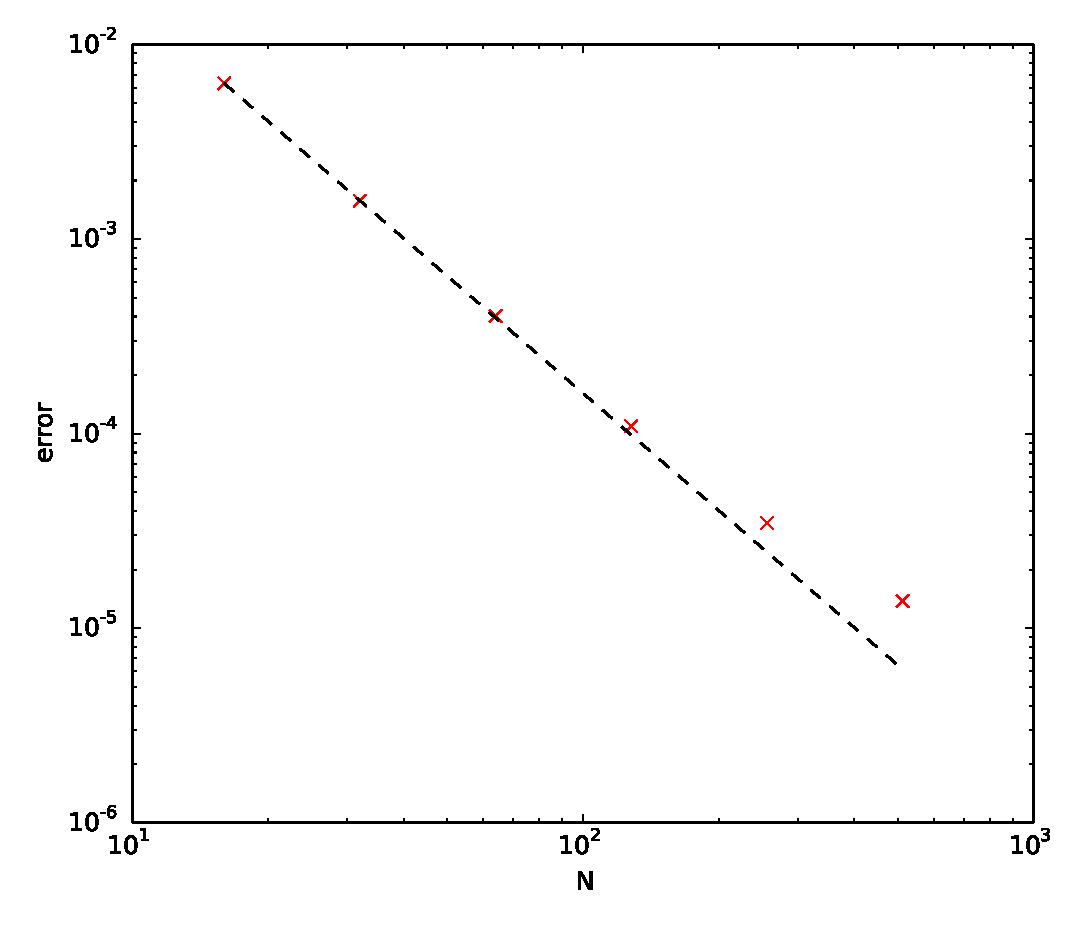
\includegraphics[width=0.8\linewidth]{mg_vc_converge}
\caption{\label{fig:mg_vc_converge} Convergence of the variable-coefficient
multigrid solver for the test problem defined in Eq.~\ref{eq:vc:lap}}.
\end{figure}

\subsubsection{Dirichlet}

We can run the same problem with Dirichlet boundary conditions on $\phi$,
and we are free to pick different boundary conditions for $\eta$, since
it represents a different physical quantity.  Since we only have homogeneous
Dirichlet or Neumann BCs implemented, we'll run with Neumann BCson $\eta$.

\section{Reactive flows}

Our constraint equation is $\nabla \cdot U = S$.  Decomposing the
velocity field as
\begin{equation}
U^\star = U^d + \frac{1}{\rho} \nabla \phi
\end{equation}
our Poisson equation can be defined by taking the divergence, and
using $\nabla \cdot U^d = S$, giving
\begin{equation}
\nabla \cdot \frac{1}{\rho} \nabla \phi = \nabla \cdot U^\star - S
\end{equation}


\section{Atmospheric flows}

Our constraint equation is $\nabla \cdot (\beta_0 U) = 0$.  Decomposing the velocity field
as 
\begin{equation}
U^\star = U^d + \frac{1}{\rho} \nabla \phi
\end{equation}
our Poisson equation can be defined by multiplying by $\beta_0$ and
taking the divergence, and using $\nabla \cdot (\beta_0 U^d) = 0$, giving
\begin{equation}
\nabla \cdot \frac{\beta_0}{\rho} \nabla \phi = \nabla \cdot (\beta_0 U^\star)
\end{equation}
